\subsection{Test di integrazione}
Questa tipologia di test serve per verificare che le varie componenti del sistema interagiscono tra loro nella maniera attesa. La strategia per definire -e poi eseguire- i seguenti test, è quella di partire dalle singole componenti per poi realizzare le varie funzionalità incrementalmente durante lo sviluppo del prodotto finale. Questo potrà essere di aiuto in caso di errori, in quanto essi si presenteranno in un ambiente già testato e funzionante. \\
Per ogni test viene specificato il suo codice univoco, la descrizione e lo stato di implementazione attuale.

	\begin{longtable}{|>{\centering\arraybackslash}m{1.6cm}|>{\centering\arraybackslash}m{6.41cm}|>{\centering\arraybackslash}m{3.1cm}|}		
		\rowcolor{LightBlue}
		\textbf{\textcolor{white}{Test}}
		& \multicolumn{1}{|c|}{\textbf{\textcolor{white}{ Descrizione}}}
		& \textbf{\textcolor{white}{Esito}}\\
		\hline
		TI1
		& Test d’integrazione front-end e back-end per la corretta visualizzazione del front-end.
		& Non implementato
		\\ \hline
		\rowcolor{LightGray}
		TI2
		& Test d’integrazione front-end e back-end per l'invio dei dati al front-end.
		& Non implementato
		\\ \hline
		TI3
		& Test d’integrazione front-end e back-end per la ricezione di dati dal front-end tramite POST.
		& Non implementato
		\\ \hline
		\rowcolor{LightGray}
		TI4
		& Test d’integrazione front-end e back-end per la ricezione di dati dal front-end tramite GET.
		& Non implementato
		\\ \hline
		TI5
		& Test d’integrazione tra back-end e Hunpos per il POS-Tagging$^*$.
		& Non implementato
		\\ \hline
		\rowcolor{LightGray}
		TI6
		& Test d’integrazione tra back-end e Hunpos per il training.
		& Non implementato
		\\ \hline	
		TI7
		& Test d’integrazione tra back-end e Google Firebase Realtime Database per la lettura dalla base di dati.
		& Non implementato
		\\ \hline	
		\rowcolor{LightGray}
		TI8
		& Test d’integrazione tra back-end e Google Firebase Realtime Database per la scrittura sulla base di dati.
		& Non implementato
		\\ \hline	
		TI9
		& Test d’integrazione tra back-end e Google Firebase Realtime Database per la modifica della base di dati.
		& Non implementato
		\\ \hline	
		\rowcolor{LightGray}
		TI10
		& Test d’integrazione tra back-end e Google Firebase Realtime Database per l'eliminazione dalla base di dati.
		& Non implementato
		\\ \hline	
		\caption{Test di integrazione}
\end{longtable}


\subsection{Test di unità}
\begin{longtable}{|>{\centering\arraybackslash}m{1.6cm}|>{\centering\arraybackslash}m{6.41cm}|>{\centering\arraybackslash}m{3.1cm}| c |}		
		\rowcolor{LightBlue}
		\textbf{\textcolor{white}{Test}}
		& \multicolumn{1}{|c|}{\textbf{\textcolor{white}{ Descrizione}}}
		& \textbf{\textcolor{white}{Stato}}
		& \textbf{\textcolor{white}{Esito}}\\
		\hline
		TU & Verifica che il metodo ritorni il nome corretto della classe su cui è richiamato. & Implementato & Superato \\ \hline
		TU & Verifica che il metodo ritorni la descrizione corretta della classe su cui è richiamato. & Implementato & Superato  \\ \hline
		TU & Verifica che venga ritornato l'id corretto dell'insegnante creatore della classe su cui il metodo è richiamato. & Implementato & Superato  \\ \hline
		TU & Verifica che venga ritornata la corretta lista di studenti appartenenti alla classe su cui il metodo è richiamato. & Implementato & Superato  \\ \hline
		TU & Verifica che venga ritornata la corretta lista di esercizi assegnati alla classe su cui il metodo è richiamato. & Implementato & Superato  \\ \hline
		TU & Verifica che ritorni il giusto numero di studenti studenti appartenenti alla classe su cui il metodo è richiamato. & Implementato & Superato  \\ \hline
		TU & Verifica che il metodo elimini correttamente uno studente dalla lista di quelli appartenenti alla classe su cui è  richiamato. & Implementato & Superato  \\ \hline
		TU & Verifica che il metodo elimini correttamente un esercizio dalla lista di quelli assegnati alla classe su cui è  richiamato. & Implementato & Superato  \\ \hline
		TU & Verifica che il metodo aggiunga correttamente uno studente dalla lista di quelli appartenenti alla classe su cui è  richiamato. & Implementato & Superato  \\ \hline
		TU & Verifica che il metodo aggiunga correttamente un esercizio dalla lista di quelli assegnati alla classe su cui è  richiamato. & Implementato & Superato  \\ \hline
		TU & Verifica che venga ritornato "true" se uno studente appartiene alla classe su cui il metodo viene richiamato; "false" altrimenti. & Implementato & Superato  \\ \hline		
		TU & Verifica che il metodo ritorni il valore della chiave dell'esercizio su cui è richiamato. & Implementato & Superato  \\ \hline
		TU & Verifica che venga ritornata la corretta frase dell'esercizio su cui il metodo è richiamato. & Implementato & Superato  \\ \hline
		TU & Verifica che venga ritornato il corretto id dell'autore dell'esercizio su cui il metodo è richiamato. & Implementato & Superato  \\ \hline
		TU & Verifica che il metodo ritorni un nuovo riferimento a POSManager. & Non implementato & Non superato \\ \hline
		TU & Verifica che venga ritornata la corretta lista di soluzioni dell'esercizio su cui il metodo è richiamato. & Non implementato & Non superato \\ \hline
		TU & Verifica che venga modificata correttamente la chiave dell'esercizio su cui il metodo è stato richiamato. & Non implementato & Non superato \\ \hline
		TU & Verifica che venga modificata correttamente la frase dell'esercizio su cui il metodo è stato richiamato. & Non implementato & Non superato \\ \hline
		TU & Verifica che venga modificata correttamente la soluzione dell'esercizio su cui il metodo è stato richiamato. & Non implementato & Non superato \\ \hline
		TU & Verifica che venga aggiunta correttamente la soluzione alla lista delle soluzioni dell'esercizio su cui il metodo è stato richiamato. & Non implementato & Non superato \\ \hline
		TU & Verifica che venga restituita correttamente la lista delle soluzioni dell'esercizio su cui il metodo è stato richiamato. & Non implementato & Non superato \\ \hline
		TU & Verifica che venga aggiunta correttamente una valutazione all'esercizio su cui il metodo è stato richiamato. & Non implementato & Non superato \\ \hline
		TU & Verifica che venga ritornata la soluzione corrente dell'esercizio su cui il metodo è richiamato. & Non implementato & Non superato \\ \hline
		TU & Verifica che venga ritornata la corretta soluzione automatica dell'esercizio su cui il metodo è richiamato. & Non implementato & Non superato \\ \hline
		TU & Verifica che venga ritornata la frase splittata dell'esercizio su cui il metodo viene richiamato. & Non implementato & Non superato \\ \hline
		TU & Verifica che venga inserita correttamente una valutazione alla soluzione corrente dell'esercizio su cui il metodo è richiamato. & Non implementato & Non superato \\ \hline		
		TU & Verifica che il metodo ritorni lo username corretto dell'utente su cui è richiamato. & Implementato & Superato \\ \hline
		TU & Verifica che il metodo ritorni il nome corretto dell'utente su cui è richiamato. & Implementato & Superato  \\ \hline
		TU & Verifica che il metodo ritorni il cognome corretto dell'utente su cui è richiamato. & Implementato & Superato  \\ \hline
		TU & Verifica che il metodo ritorni la città corretta dell'utente su cui è richiamato. & Implementato & Superato  \\ \hline
		TU & Verifica che il metodo ritorni la scuola corretta dell'utente su cui è richiamato. & Implementato & Superato  \\ \hline
		TU & Verifica che il metodo ritorni la password corretta dell'utente su cui è richiamato. & Implementato & Superato  \\ \hline
		TU & Verifica che il metodo ritorni "true" se vi è corrispondenza tra la prima e seconda password inserita dallo studente in fase di registrazione; "false" altrimenti. & Implementato & Superato  \\ \hline
		TU & Verifica che il metodo ritorni l'id corretto dell'utente su cui è richiamato. & Implementato & Superato  \\ \hline
		TU & Verifica che il metodo ritorni l'id modificato correttamente dello studente su cui è richiamato. & Implementato & Superato  \\ \hline
		TU & Verifica che il metodo ritorni "false" se l'utente su cui è richiamato è uno studente, "true" se è un insegnante. & Implementato & Superato \\ \hline
		TU & Verifica che venga ritornata la corretta lista delle classi a cui appartiene lo studente o create dall'insegnante su cui il metodo è richiamato. & Implementato & Superato \\ \hline
		TU & Verifica che il metodo ritorni la corretta media dello studente su cui è richiamato. & Implementato & Superato  \\ \hline
		TU & Verifica che il metodo ritorni il codice INPS corretto dell'insegnante su cui è richiamato. & Implementato & Superato  \\ \hline
		TU & Verifica che il metodo ritorni il valore della chiave della soluzione su cui è richiamato. & Non implementato & Non superato \\ \hline
		TU & Verifica che il metodo ritorni l'id dell'autore della soluzione su cui è richiamato.& Non implementato & Non superato \\ \hline
		TU & Verifica che il metodo ritorni gli argomenti della soluzione su cui è richiamato. & Non implementato & Non superato \\ \hline
		TU & Verifica che il metodo ritorni la difficoltà della soluzione su cui è richiamato. & Non implementato & Non superato \\ \hline
		TU & Verifica che il metodo ritorni i tag della soluzione su cui è richiamato. & Non implementato & Non superato \\ \hline
		TU & Verifica che il metodo ritorni le valutazioni della soluzione su cui è richiamato. & Non implementato & Non superato \\ \hline
		TU & Verifica che il metodo ritorni le valutazioni della soluzione su cui è richiamato in formato JSON. & Non implementato & Non superato \\ \hline
		TU & Verifica che il metodo ritorni la data della soluzione su cui è richiamato & Non implementato & Non superato \\ \hline
		TU & Verifica che il metodo aggiunga correttamente una valutazione alla soluzione su cui è richiamato & Non implementato & Non superato \\ \hline
		TU & Verifica che il metodo ritorni una valutazione tra 0 e 10 della soluzione su cui è richiamato & Non implementato & Non superato \\ \hline
		\caption{Test di unità}
\end{longtable}

\subsubsection{Tracciamento test di unità}
\begin{longtable}{|>{\centering\arraybackslash}m{1.6cm}|c|}		
 	\rowcolor{LightBlue}
		\textbf{\textcolor{white}{Test}}
		& \textbf{\textcolor{white}{Metodo}}\\		\hline
		TU & ClassTest.getName()\\ \hline
		TU & ClassTest.getDescription()\\ \hline
		TU & ClassTest.getTeacherID()\\ \hline
		TU & ClassTest.getStudents()\\ \hline
		TU & ClassTest.getExercises()\\ \hline
		TU & ClassTest.getNumberOfStudents()\\ \hline
		TU & ClassTest.deleteStudent()\\ \hline
		TU & ClassTest.deleteExercise()\\ \hline
		TU & ClassTest.addStudent()\\ \hline
		TU & ClassTest.addExercise()\\ \hline
		TU & ClassTest.findStudent()\\ \hline
		TU & ExerciseTest.getKey()\\ \hline
		TU & ExerciseTest.getSentence()\\ \hline
		TU & ExerciseTest.getAuthorId()\\ \hline
		TU & ExerciseTest.getPOSManager()\\ \hline
		TU & ExerciseTest.setKey()\\ \hline
		TU & ExerciseTest.setSentence()\\ \hline
		TU & ExerciseTest.setSolution()\\ \hline
		TU & ExerciseTest.addSolution()\\ \hline
		TU & ExerciseTest.getSolution()\\ \hline
		TU & ExerciseTest.addValutation()\\ \hline
		TU & ExerciseTest.getNewSolution()\\ \hline
		TU & ExerciseTest.autosolve()\\ \hline
		TU & ExerciseTest.getSplitSentence()\\ \hline
		TU & ExerciseTest.evaluate(teacherID : string)\\ \hline
		TU & StudentTest.getUsername()\\ \hline
		TU & StudentTest.getName()\\ \hline
		TU & StudentTest.getLastName()\\ \hline
		TU & StudentTest.getCity()\\ \hline
		TU & StudentTest.getSchool()\\ \hline
		TU & StudentTest.getPassword()\\ \hline
		TU & StudentTest.samePassword()\\ \hline
		TU & StudentTest.getID()\\ \hline
		TU & StudentTest.setID()\\ \hline
		TU & StudentTest.isTeacher()\\ \hline
		TU & StudentTest.getClasses()\\ \hline
		TU & StudentTest.getAverage()\\ \hline
		TU & StudentTest.isTeacher()\\ \hline
		TU & SolutionTest.getKey()\\ \hline
		TU & SolutionTest.getSolverId()\\ \hline
		TU & SolutionTest.getTopics()\\ \hline
		TU & SolutionTest.getDifficulty()\\ \hline
		TU & SolutionTest.getSolutionTags()\\ \hline
		TU & SolutionTest.getValutations()\\ \hline
		TU & SolutionTest.JSONValutations()\\ \hline
		TU & SolutionTest.getTime()\\ \hline
		TU & SolutionTest.addNewMark(teacherID : string, mark : number)\\ \hline
		TU & SolutionTest.evaluateSolution(tags: string [])\\ \hline
		\caption{Tracciamento test di unità}
\end{longtable}

	
\newpage
\section{Resoconto attività di verifica}
\subsection{Prodotto}
\subsubsection{Documentazione}
Nella tabella seguente vengono riportati i risultati delle verifiche eseguite sui documenti. Il resoconto contiene le verifiche sia dei documenti esterni, cioè utili al committente, sia interni, utili invece al team Ottobit.\\
	\begin{longtable}{>{\centering\arraybackslash}m{5cm} >{\centering\arraybackslash}m{4cm} >{\centering\arraybackslash}m{5cm} >{\centering\arraybackslash}m{2cm}}
		\rowcolor{LightBlue}
		\textbf{\textcolor{white}{Documento}}
		& \textbf{\textcolor{white}{Indice Gulpease}}
		& \textbf{\textcolor{white}{Esito}}\\
		\textit{StudioDiFattibilità\_v1.0.0} & 60 & Accettato\\
		\hline
		\rowcolor{LightGray}
		\textit{AnalisiDeiRequisiti\_v1.0.0} & 82 & Accettato\\
		\hline
		\textit{NormeDiProgetto\_v1.0.0} & 67 & Accettato\\
		\hline
		\rowcolor{LightGray}
		\textit{PianoDiQualifica\_v1.0.0} & 72 & Accettato\\
		\hline
		\textit{PianoDiProgetto\_v1.0.0} & 64 & Accettato\\
		\hline
		\caption{Resoconto attività di verifica per la revisione dei requisiti}
	\end{longtable}
	
	\begin{longtable}{>{\centering\arraybackslash}m{5cm} >{\centering\arraybackslash}m{4cm} >{\centering\arraybackslash}m{5cm} >{\centering\arraybackslash}m{2cm}}
		\rowcolor{LightBlue}
		\textbf{\textcolor{white}{Documento}}
		& \textbf{\textcolor{white}{Indice Gulpease}}
		& \textbf{\textcolor{white}{Esito}}\\
		\textit{StudioDiFattibilità\_v1.0.0} & 60 & Accettato\\
		\hline
		\rowcolor{LightGray}
		\textit{AnalisiDeiRequisiti\_v2.0.0} & 82 & Accettato\\
		\hline
		\textit{NormeDiProgetto\_v2.0.0} & 69 & Accettato\\
		\hline
		\rowcolor{LightGray}
		\textit{PianoDiQualifica\_v2.0.0} & 72 & Accettato\\
		\hline
		\textit{PianoDiProgetto\_v2.0.0} & 64 & Accettato\\
		\hline
		\caption{Resoconto attività di verifica per la revisione di progettazione}
	\end{longtable}


\subsubsection{Software}
Le metriche per il software non vengono calcolate fino all'inizio dell'attività di codifica. Nei processi precedenti, nonostante si sia iniziato a scrivere del codice (in funzione dello sviluppo di un \textit{Proof of Concept}$^*$), questo non viene considerato nel calcolo delle metriche.

\subsection{Processi}
\subsubsection{Valori ISO/IEC 15504 - MPC1}

Riportiamo di seguito i grafici rappresentanti il livello raggiunto alla data di ogni revisione dai vari processi.


\begin{figure}[H]
	\centering
	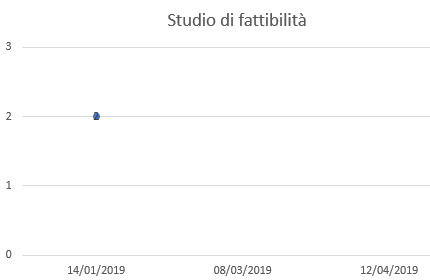
\includegraphics[scale=1]{images/resoconto/Studio.png}
	\caption{Valori ISO/IEC 15504 - Studio di fattibilità}	
\end{figure}


\begin{figure}[H]
	\centering
	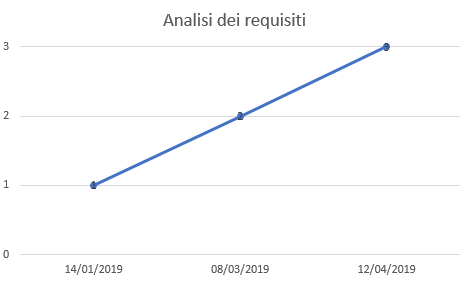
\includegraphics[scale=1]{images/resoconto/Analisi.png}
	\caption{Valori ISO/IEC 15504 - Analisi dei Requisiti}	
\end{figure}


\begin{figure}[H]
	\centering
	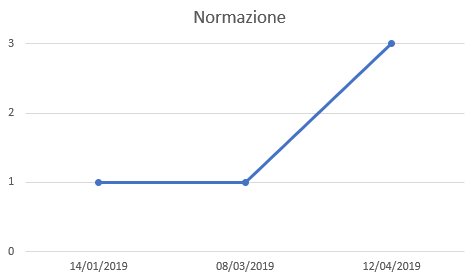
\includegraphics[scale=1]{images/resoconto/Normazione.png}
	\caption{Valori ISO/IEC 15504 - Normazione}	
\end{figure}


\begin{figure}[H]
	\centering
	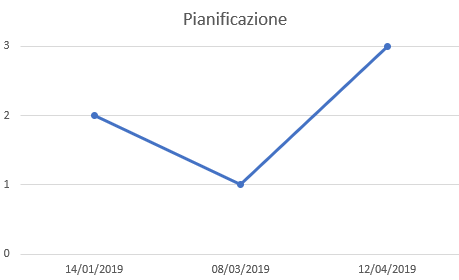
\includegraphics[scale=1]{images/resoconto/Pianificazione.png}
	\caption{Valori ISO/IEC 15504 - Pianificazione}	
\end{figure}


\begin{figure}[H]
	\centering
	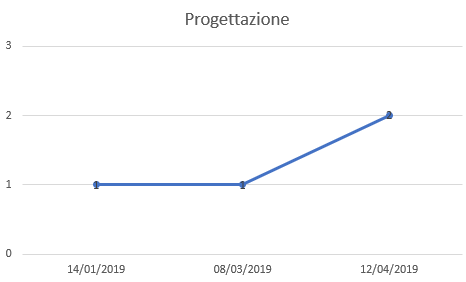
\includegraphics[scale=1]{images/resoconto/Progettazione.png}
	\caption{Valori ISO/IEC 15504 - Progettazione}	
\end{figure}


\begin{figure}[H]
	\centering
	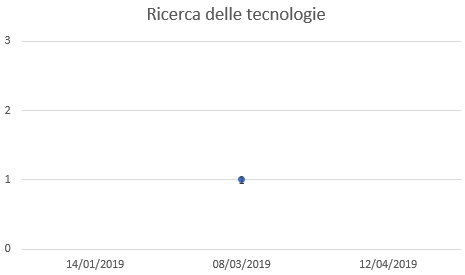
\includegraphics[scale=1]{images/resoconto/Ricerca.png}
	\caption{Valori ISO/IEC 15504 - Ricerca delle tecnologie}	
\end{figure}


\begin{figure}[H]
	\centering
	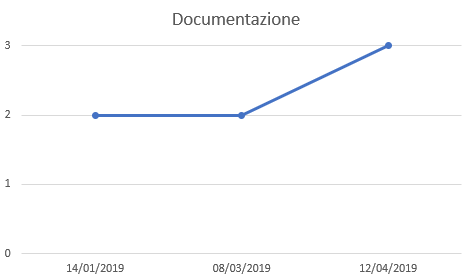
\includegraphics[scale=1]{images/resoconto/Documentazione.png}
	\caption{Valori ISO/IEC 15504 - Documentazione}	
\end{figure}


\begin{figure}[H]
	\centering
	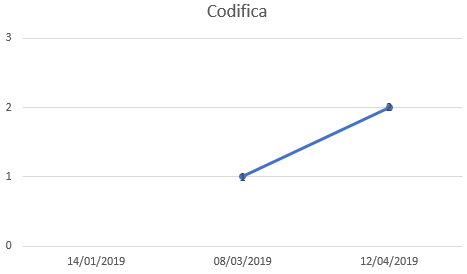
\includegraphics[scale=1]{images/resoconto/Codifica.png}
	\caption{Valori ISO/IEC 15504 - Codifica}	
\end{figure}

\paragraph{Revisione di progetto\\}
Durante il periodo di Revisione di progetto abbiamo individuato periodicamente tutti i cambiamenti apportati ai requisiti del progetto. Questo ci ha permesso di determinare la stabilità dei requisiti nel tempo grazie all'utilizzo della metrica MPC2.
Riportiamo di seguito i calcoli e le varie rilevazioni effettuate.

\begin{longtable}{>{\centering\arraybackslash}m{3cm} >{\centering\arraybackslash}m{4cm} >{\centering\arraybackslash}m{5cm} >{\centering\arraybackslash}m{2cm}}
	\rowcolor{LightBlue}
	\textbf{\textcolor{white}{Data rilevazioni}}
	& \textbf{\textcolor{white}{Requirement Stability Index (RSI)}}
	& \textbf{\textcolor{white}{Esito}}\\
	
	2019-02-15 & \[1-\frac{0+5+4}{48}=0.81\] & Accettato\\
	\hline
	2019-02-20 & \[1-\frac{5+0+3}{43}=0.81\] & Accettato\\
	\hline
	2019-02-21 & \[1-\frac{8+0+3}{48}=0.77\] & Accettato\\
	\hline
	2019-02-22 & \[1-\frac{5+2+0}{56}=0.85\] & Accettato\\
	\hline
	2019-02-25 & \[1-\frac{11+0+0}{59}=0.81\] & Accettato\\
	\hline
	2019-02-27 & \[1-\frac{10+0+0}{70}=0.88\] & Accettato\\
	\hline
	2019-03-04 & \[1-\frac{12+0+0}{80}=0.86\] & Accettato\\
	\hline
	2019-03-05 & \[1-\frac{14+0+1}{92}=0.83\] & Accettato\\
	\hline\\
	\caption{Rilevazioni indice stabilità requisiti (RSI) - Revisione di progetto}
\end{longtable}
\begin{figure}[H]
	\centering
	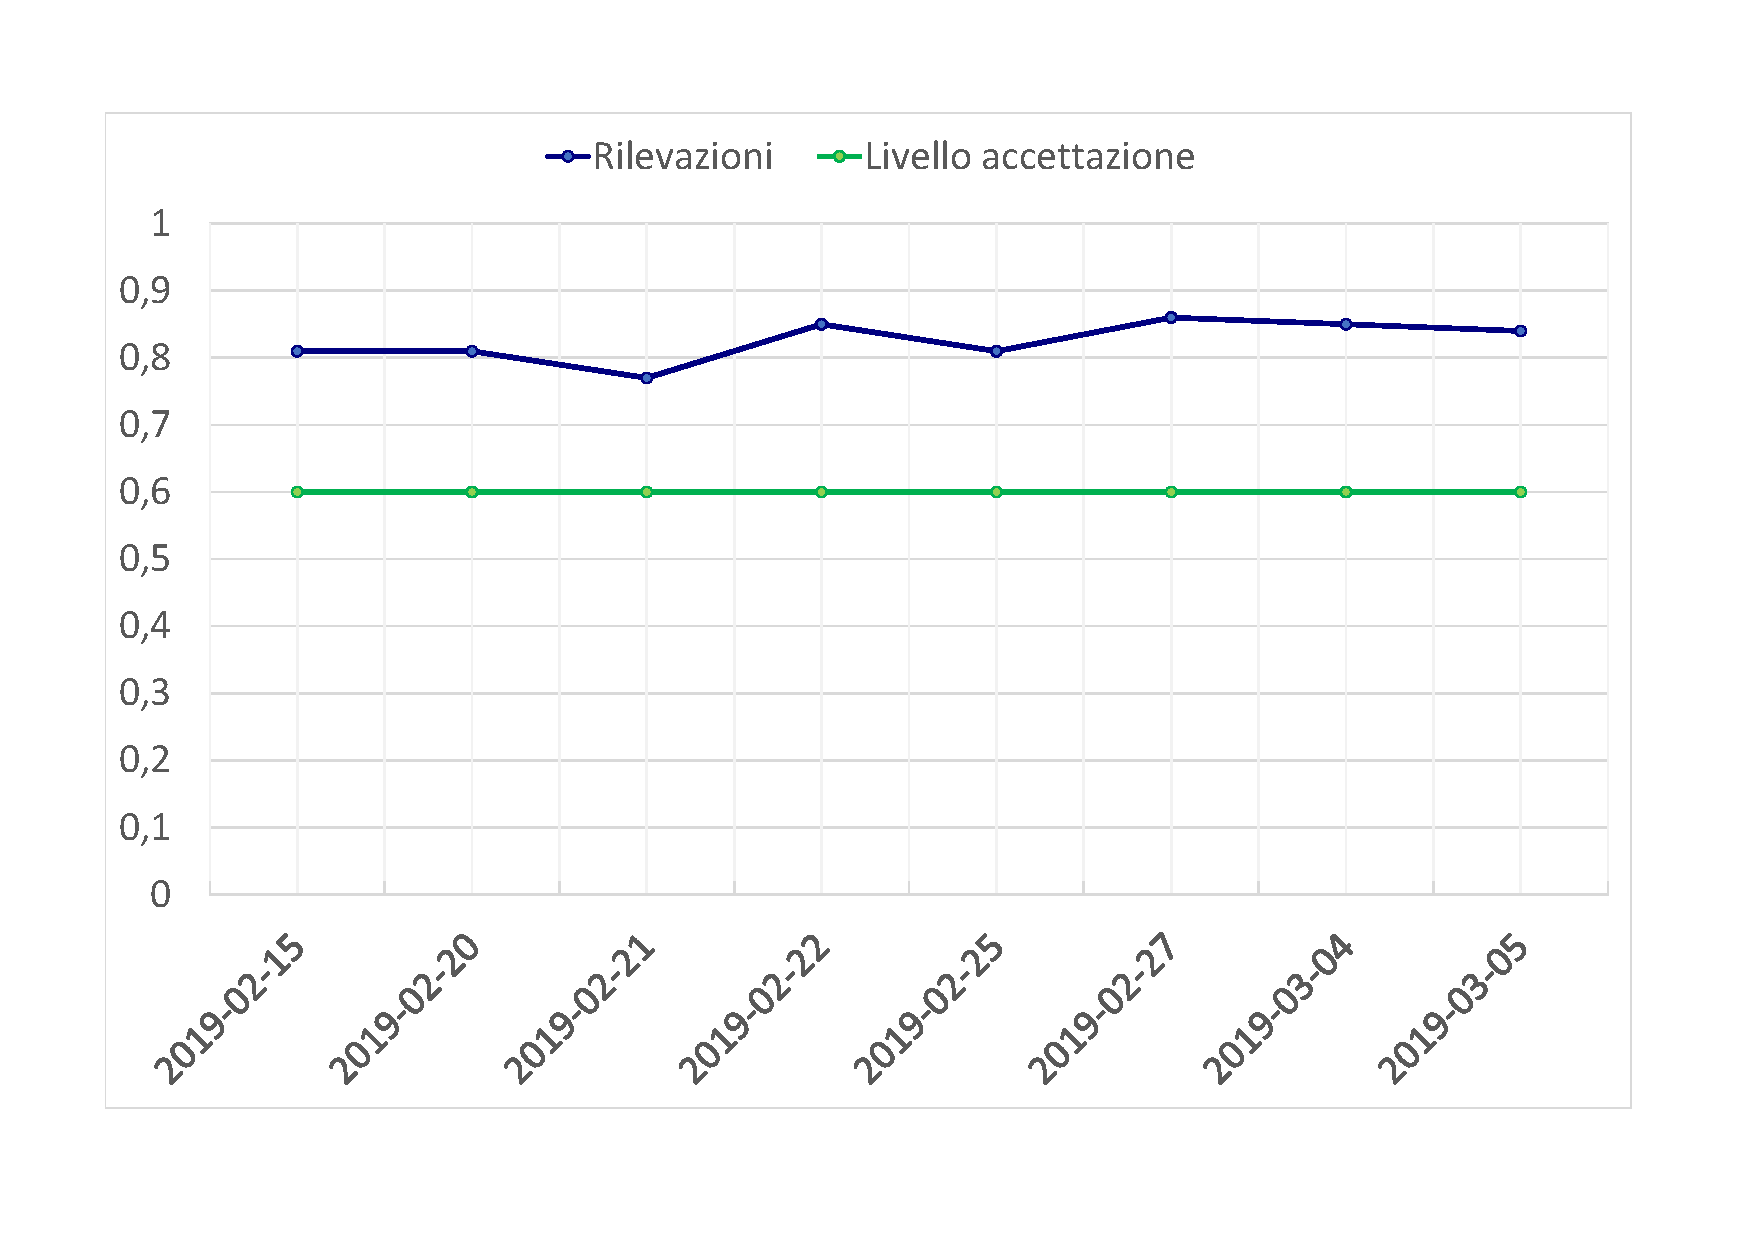
\includegraphics[scale=0.6]{images/resoconto/requisitiChart.pdf}
	\caption{Serie storica rilevazioni stabilità requisiti - Revisione di progetto}	
\end{figure}

\subsection{Esito delle revisioni - RR}
Successivamente alla prima revisione formale, il gruppo ha apportato diverse modifiche ai documenti basandosi sulle osservazioni ricevute dai docenti. Le modifiche sono riassunte di seguito:
	\begin{itemize}
		\item \textbf{Norme di Progetto}: è stata aggiunta una sezione riportante le metriche di riferimento per processi e prodotti e la relativa normazione. 
		\item \textbf{Piano di Progetto}: le attività sono state ripianificate a partire dalla fase 2 ed è stato redatto un nuovo consuntivo.
		\item \textbf{Piano di Qualifica}: la struttura del documento è stata completamente rivista, i contenuti sono stati modificati secondo le indicazioni riportate nell'esito della prima revisione. Sono stati aggiunti diversi tipi di test e diverse appendici con argomenti vari; sono stati stabiliti degli obiettivi di qualità.
		\item \textbf{Analisi dei Requisiti}: sono stati aggiunti diversi nuovi casi d'uso, specializzando quelli già presenti e raddoppiandone il numero; sono stati modificati i diagrammi UML. \`E stata aggiunta una sezione introduttiva ed una descrizione degli attori implicati nel progetto. 
	\end{itemize}

\subsection{Esito delle revisioni - RP}	
Successivamente alla seconda revisione formale, il gruppo ha apportato diverse modifiche ai documenti basandosi sulle osservazioni ricevute dai docenti. Le modifiche sono riassunte di seguito:
	\begin{itemize}
		\item \textbf{Norme di Progetto}: sono state aggiunte diverse norme ed attività al processo di fornitura, revisionando contestualmente quelle già inserite. Sono state rimosse le soglie associate ad ogni metrica e la struttura del documento è stata in parte rivisitata.
		\item \textbf{Piano di Progetto}: le fasi 3 e 4 sono state ripianificate sulla base del periodo precedente; si è cercato di dare maggiore spessore all'incrementalità della logica di sviluppo adottata. 
		\item \textbf{Piano di Qualifica}: la struttura del documento è stata revisionata, sono stati redatti i test di unità e si è cercato di dare una struttura a cruscotto ai riscontri di verifica.
		\item \textbf{Analisi dei Requisiti}: i casi d'uso sono stati rivisti, aumentandone quanto possibile il livello di dettaglio; i codici dei casi d'uso e dei requisiti sono stati modificati e, di conseguenza, hanno subito modifiche anche i diagrammi UML.
	\end{itemize}

\newpage
\section{Copertura dei requisiti}
Viene riportata in seguito una tabella riassuntiva dei requisiti che non è da considerarsi definitiva, verrà infatti aggiornata in seguito ad ogni avanzamento significativo. \\
I requisiti sono indicati con il loro codice identificativo definito nel documento \textit{NormeDiProgetto\_v2.0.0} e la loro descrizione dettagliata è riportata nel documento \textit{AnalisiDeiRequisiti\_v2.0.0}.
\begin{longtable}{| p{2.5cm} | p{3cm} |}
	\rowcolor{LightBlue}
	\color{white}\bfseries Requisito & \color{white}\bfseries Stato \\
	ROF1 & Non soddisfatto \\ \hline
	ROF2 & Non soddisfatto \\ \hline
	ROF3 & Non soddisfatto \\ \hline
	ROF4 & Non soddisfatto \\ \hline
	ROF5 & Non soddisfatto \\ \hline
	ROF6 & Non soddisfatto \\ \hline
	ROF7 & Non soddisfatto \\ \hline
	ROF8 & Non soddisfatto \\ \hline
	ROF9 & Non soddisfatto \\ \hline
	ROF10 & Non soddisfatto \\ \hline
	ROF11 & Non soddisfatto \\ \hline
	ROF12 & Non soddisfatto \\ \hline
	ROF13 & Non soddisfatto \\ \hline
	ROF14 & Non soddisfatto \\ \hline
	ROF15 & Non soddisfatto \\ \hline
	ROF16 & Non soddisfatto \\ \hline
	ROF17 & Non soddisfatto \\ \hline
	ROF18 & Non soddisfatto \\ \hline
	ROF19 & Non soddisfatto \\ \hline
	ROF20 & Non soddisfatto \\ \hline
	ROF21 & Non soddisfatto \\ \hline
	ROF22 & Non soddisfatto \\ \hline
	ROF23 & Non soddisfatto \\ \hline
	ROF24 & Non soddisfatto \\ \hline
	ROF25 & Non soddisfatto \\ \hline
	ROF26 & Non soddisfatto \\ \hline
	ROF27 & Non soddisfatto \\ \hline
	ROF28 & Non soddisfatto \\ \hline
	ROF29 & Non soddisfatto \\ \hline
	ROF30 & Non soddisfatto \\ \hline
	ROF31 & Non soddisfatto \\ \hline
	ROF32 & Non soddisfatto \\ \hline
	ROF33 & Non soddisfatto \\ \hline
	ROF34 & Non soddisfatto \\ \hline
	RDF1 & Non soddisfatto \\ \hline
	RDF2 & Non soddisfatto \\ \hline
	RDF3 & Non soddisfatto \\ \hline
	RDF4 & Non soddisfatto \\ \hline
	RDF5 & Non soddisfatto \\ \hline
	RDF6 & Non soddisfatto \\ \hline
	RDF7 & Non soddisfatto \\ \hline
	RDF8 & Non soddisfatto \\ \hline
	RDF9 & Non soddisfatto \\ \hline
	RDF10 & Non soddisfatto \\ \hline
	RDF11 & Non soddisfatto \\ \hline
	RDF12 & Non soddisfatto \\ \hline
	RDF13 & Non soddisfatto \\ \hline
	RDF14 & Non soddisfatto \\ \hline
	RDF15 & Non soddisfatto \\ \hline
	RDF16 & Non soddisfatto \\ \hline
	RDF17 & Non soddisfatto \\ \hline
	RDF18 & Non soddisfatto \\ \hline
	RDF19 & Non soddisfatto \\ \hline
	RDF20 & Non soddisfatto \\ \hline
	RDF21 & Non soddisfatto \\ \hline
	RDF22 & Non soddisfatto \\ \hline
	RDF23 & Non soddisfatto \\ \hline
	RDF24 & Non soddisfatto \\ \hline
	RDF25 & Non soddisfatto \\ \hline
	RDF26 & Non soddisfatto \\ \hline
	RDF27 & Non soddisfatto \\ \hline
	RDF28 & Non soddisfatto \\ \hline
	RDF29 & Non soddisfatto \\ \hline
	RPF1 & Non soddisfatto \\ \hline
	RPF2 & Non soddisfatto \\ \hline
	RPF3 & Non soddisfatto \\ \hline
	RPF4 & Non soddisfatto \\ \hline
	RPF5 & Non soddisfatto \\ \hline
	RPF6 & Non soddisfatto \\ \hline
	RPF7 & Non soddisfatto \\ \hline
	RPF8 & Non soddisfatto \\ \hline
	RPF9 & Non soddisfatto \\ \hline
	RPF10 & Non soddisfatto \\ \hline
	RPF11 & Non soddisfatto \\ \hline
	RPF12 & Non soddisfatto \\ \hline
	RPF13 & Non soddisfatto \\ \hline
	RPF14 & Non soddisfatto \\ \hline
	RPF15 & Non soddisfatto \\ \hline
	RPF16 & Non soddisfatto \\ \hline
	RPF17 & Non soddisfatto \\ \hline
	RPF18 & Non soddisfatto \\ \hline
	RPF19 & Non soddisfatto \\ \hline
	RPF20 & Non soddisfatto \\ \hline
	RPF21 & Non soddisfatto \\ \hline
	RPF22 & Non soddisfatto \\ \hline
	RPF23 & Non soddisfatto \\ \hline
	RPF24 & Non soddisfatto \\ \hline
	RPF25 & Non soddisfatto \\ \hline
	RPF26 & Non soddisfatto \\ \hline
	RPF27 & Non soddisfatto \\ \hline
	RPF28 & Non soddisfatto \\ \hline
	ROV1 & Non soddisfatto \\ \hline
	ROV2 & Non soddisfatto \\ \hline
	ROV3 & Non soddisfatto \\ \hline
	ROV4 & Non soddisfatto \\ \hline
	ROV5 & Non soddisfatto \\ \hline
	RDV1 & Non soddisfatto \\ \hline
	RPV1 & Non soddisfatto \\ \hline
	ROQ1 & Non soddisfatto \\ \hline
	ROQ2 & Non soddisfatto \\ \hline
	ROQ3 & Non soddisfatto \\ \hline
	RDQ1 & Non soddisfatto \\ \hline
	RDQ2 & Non soddisfatto \\ \hline
	RDQ3 & Non soddisfatto \\ \hline
	RDQ4 & Non soddisfatto \\ \hline
	RDQ5 & Non soddisfatto \\ \hline
	RPQ1 & Non soddisfatto \\ \hline
	\caption{Riassunto copertura requisiti}
\end{longtable}


	
